\chapter{Anforderungen}\label{sec:anforderungen}

(Joshua)

In diesem Kapitel sollen die Anforderungen an die zu erstellende Applikation, sowie der zu erreichende Scope beschrieben werden um eine abschließende Bewertung durchführen zu können, die das Erreichte mit den Zielen vergleicht.

\vspace{0.25cm}

Zuerst wird die Begrifflichkeit Anforderung geklärt. In der Softwareentwicklung gibt es einige verschiedene Definitionen von \enquote{Anforderungen}. In dieser Arbeit soll der Definition gefolgt werden, welche von Helmut Balzert in seinem Buch zu den Basiskonzepten und des Requirements Engineering erarbeitet wurden \cite{Balzert.2009}. In seinem Werk werden Anforderungen wie folgt definiert.

\begin{defStrich}[Anforderungen]
	\enquote{Anforderungen (requirements) legen fest, was man von einem
		Softwaresystem als Eigenschaften erwartet}\cite{Balzert.2009} (Seite 455). Mit der Annahme, dass \enquote{man} alle Stakeholder (Personen, die ein Interesse an der Entwicklung und/oder der erstellten Software haben) beinhaltet. \cite{Balzert.2009}
\end{defStrich} 

Des Weiteren sollten vor der Festlegung der Anforderungen \enquote{Visionen und Ziele} und die Rahmenbedingungen, in denen die Software existieren sollen, festgelegt werden. Erst danach sollten Eigenschaften, welche in funktionale und nicht-funktionale Eigenschaften unterteilt werden können, definiert werden. In den folgenden Unterkapiteln wird nach diesem Prinzip vorgegangen, um eine konsistente und sinnvolle Anforderungslage zu schaffen.

\section{Visionen und Ziele}
An erster Stelle der Anforderungen steht eine Vision für das zu erstellende Produkt. In diesem Fall wurden bereits einige wichtige Punkte in der Einleitung der Arbeit zusammen gefasst, die zu einer kurzen und prägnanten Vision führen:

\vspace{0.25cm}

\enquote{Durch \textit{Travlyn} sollen Nutzer in der Lage sein, ihre Städtereisen ohne das Mitführen von papierbasierten Reiseführern oder die Nutzung von multiplen mobilen Diensten zu bewältigen, ohne dabei einen Informationsverlust oder eine Beeinträchtigung des Reisespaßes hinnehmen zu müssen.}

\vspace{0.25cm}

Anhand dieser Version, die beschreibt, was erreicht werden soll aber nicht wie, werden konkrete Ziele abgeleitet. Es wurde entschieden, dass diese Ziele dem \enquote{SMART} Prinzip folgen sollten.

\begin{defStrich}[SMART Ziele]
	Die Art und Weise messbare Ziele zu setzen kann einer festgelegten Struktur folgen. In diesem Fall soll die Struktur, welche Peter Drucker in seinem Buch \enquote{The Practice of Management} (1954) erarbeitet hat, genutzt werden. Allerdings hat Drucker nie eine genaue Erklärung zu der Bedeutung des Akronyms \enquote{SMART} abgegeben, deswegen wird folgende allgemein akzeptierte Vaiante gewählt \cite{Lawlor.2012}:
	\begin{itemize}
		\item Specific (Spezifisch)
		\item Measurable (Messbar)
		\item Attainable (Attraktiv)
		\item Realistic (Realistisch)
		\item Timely (Terminiert)
	\end{itemize}   
\end{defStrich} 

Folgend diesem Prinzip sind folgende Ziele entstanden:

\begin{itemize}
	\item Ein Nutzer soll sich vor einer Reise über \textit{Travlyn} folgende Informationen zu seiner Zielstadt einholen können: Name, Lage, Beschreibung und ein Bild, welches einen ersten Eindruck der Stadt vermittelt.
	\item Die vermittelten Informationen und durchgeführten Schritte zum Entwurf einer Reise werden anhand der vom Nutzer zur Verfügung gestellten Informationen personalisiert. Außerdem kann jeder Nutzer seine persönliche Reise designen und muss sich damit nicht auf festgelegte Routen beschränken, was zu einer hohen Individualisierung führt. 
	\item Vor und während der Reise wird \textit{Travlyn} den Nutzer entlang einer vorher festlegten Route durch die Stadt leiten und Informationen, wie Beschreibungen, Bilder und Kosten anzeigen. Die Route beinhaltet Stops an interessanten Orten der Stadt, wie Sehenswürdigkeiten und spannenden Aktivitäten.
	\item Der Nutzer kann Reisepläne teilen und Pläne von anderen Nutzern einsehen können, um sich inspirieren zu lassen und seinen eigenen Plan an den existierenden Plänen orientieren zu können. 
\end{itemize}

\section{Rahmenbedingungen}
Laut Balzert stellen Rahmenbedingungen \enquote{organisatorische und/oder technische Restriktionen für das Softwaresystem und/oder den Entwicklungsprozess} da \cite{Balzert.2009} (Seite 459).

\subsection{Organisatorisches}
Für \textit{Travyln} liegen folgende organisatorische Rahmenbedingungen vor: Der Anwendungsbereich der Software liegt im privaten Umfeld, genauer gesagt im Bereich des privaten Reisens. Die Zielgruppe sind alle Personen, die für relativ kurze Zeiträume in größere Städte reisen und diese mit ihren Sehenswürdigkeiten entdecken wollen und sich zu diesen weiter informieren wollen. Damit liegt eine mobile Benutzung unter ständiger Beobachtung des Nutzers vor. Während der Reise/der durch \textit{Travyln} geführten Tour wird die Anwendung ohne Unterbrechung laufen.

\subsection{Technisches}

Die technischen Anforderungen werden an dieser Stelle in zwei Abschnitte aufgeteilt, da sich die Rahmenbedingungen für den Server und den Client stark unterscheiden. 

\vspace{0.25cm}

Für den Server wird festgelegt, dass er in einem Docker-Container\cite{Turnbull.2014} läuft, welcher unabhängig von dem darunterliegendem Betriebssystem ist. Peripherie wird es an diesem Rechner keine geben, da er nur per Remote Zugriff von außen gesteuert werden wird. Die wichtigste Rahmenbedingung ist, dass die Hardware, auf welcher der Server läuft ständig mit dem Internet verbunden sein muss, um eine dauerhafte Verfügbarkeit zu gewährleisten

\vspace{0.25cm}

Für den Client wird festgelegt, dass er auf einem mobilen Smartphone, welches im Akkubetrieb operiert, läuft. Auf dem Gerät muss Android als Betriebssystem laufen und die Version soll 8.0 (Oreo) nicht unterschreiten. Das Gerät stellt eine klassische mobile Peripherie zur Verfügung, welche z.B. eine virtuelle Tastatur, einen GPS-Sensor und einen Lautsprecher/Kopfhöreranschluss beinhaltet. Auch für den Client muss eine konstante Internetverbindung existieren, um sicher zu stellen, dass der Server ständig erreicht werden kann und die entsprechenden Informationen abgefragt werden können.

\section{Geforderte Eigenschaften}
Nachdem die Ziele und die Rahmenbedingungen definiert sind, können die erwarteten Eigenschaften erarbeitet werden. Bei jeder Eigenschaft sollte geprüft werden, ob diese im Sinne eines der gesteckten Ziele sind und zum Erreichen der Vision beitragen und ob diese im Sinne der Rahmenbedingungen erreichbar und realistisch ist. Wenn eine dieser beiden Prüfungen nicht positiv erfüllt wird, sollte über eine Redefinition der Eigenschaft nachgedacht werden, denn in der aktuellen Form ist sie nicht zielführend und kann mit dem vorliegendem Rahmen ggf. nicht umgesetzt werden.

\vspace{0.25cm}

Wie im vorherigen Verlauf beschreiben, werden Eigenschaften häufig in funktional und nicht-funktional aufgeteilt \cite{Balzert.2009}. Im Folgenden wird dieser Trennung gefolgt.

\newpage

\subsection{Funktionale Eigenschaften}\label{sec:funktionale_eigenschaften}
\label{sec:funcReq}
Unter funktionalen Eigenschaften wird alles spezifiziert, was ein System tun und explizit nicht tun/können soll. Laut Balzert können diese Eigenschaften in statische, dynamische und logische Eigenschaften aufgeteilt werden\cite{Balzert.2009}. Wir haben uns explizit gegen eine solche Gliederung entschieden, um dieses Kapitels nicht zu sprengen.

\vspace{0.25cm}

Zur Visualisierung der erwarteten funktionalen Eigenschaften wurde ein Use Case Diagramm erstellt.
\begin{figure}[H]
	\centering
	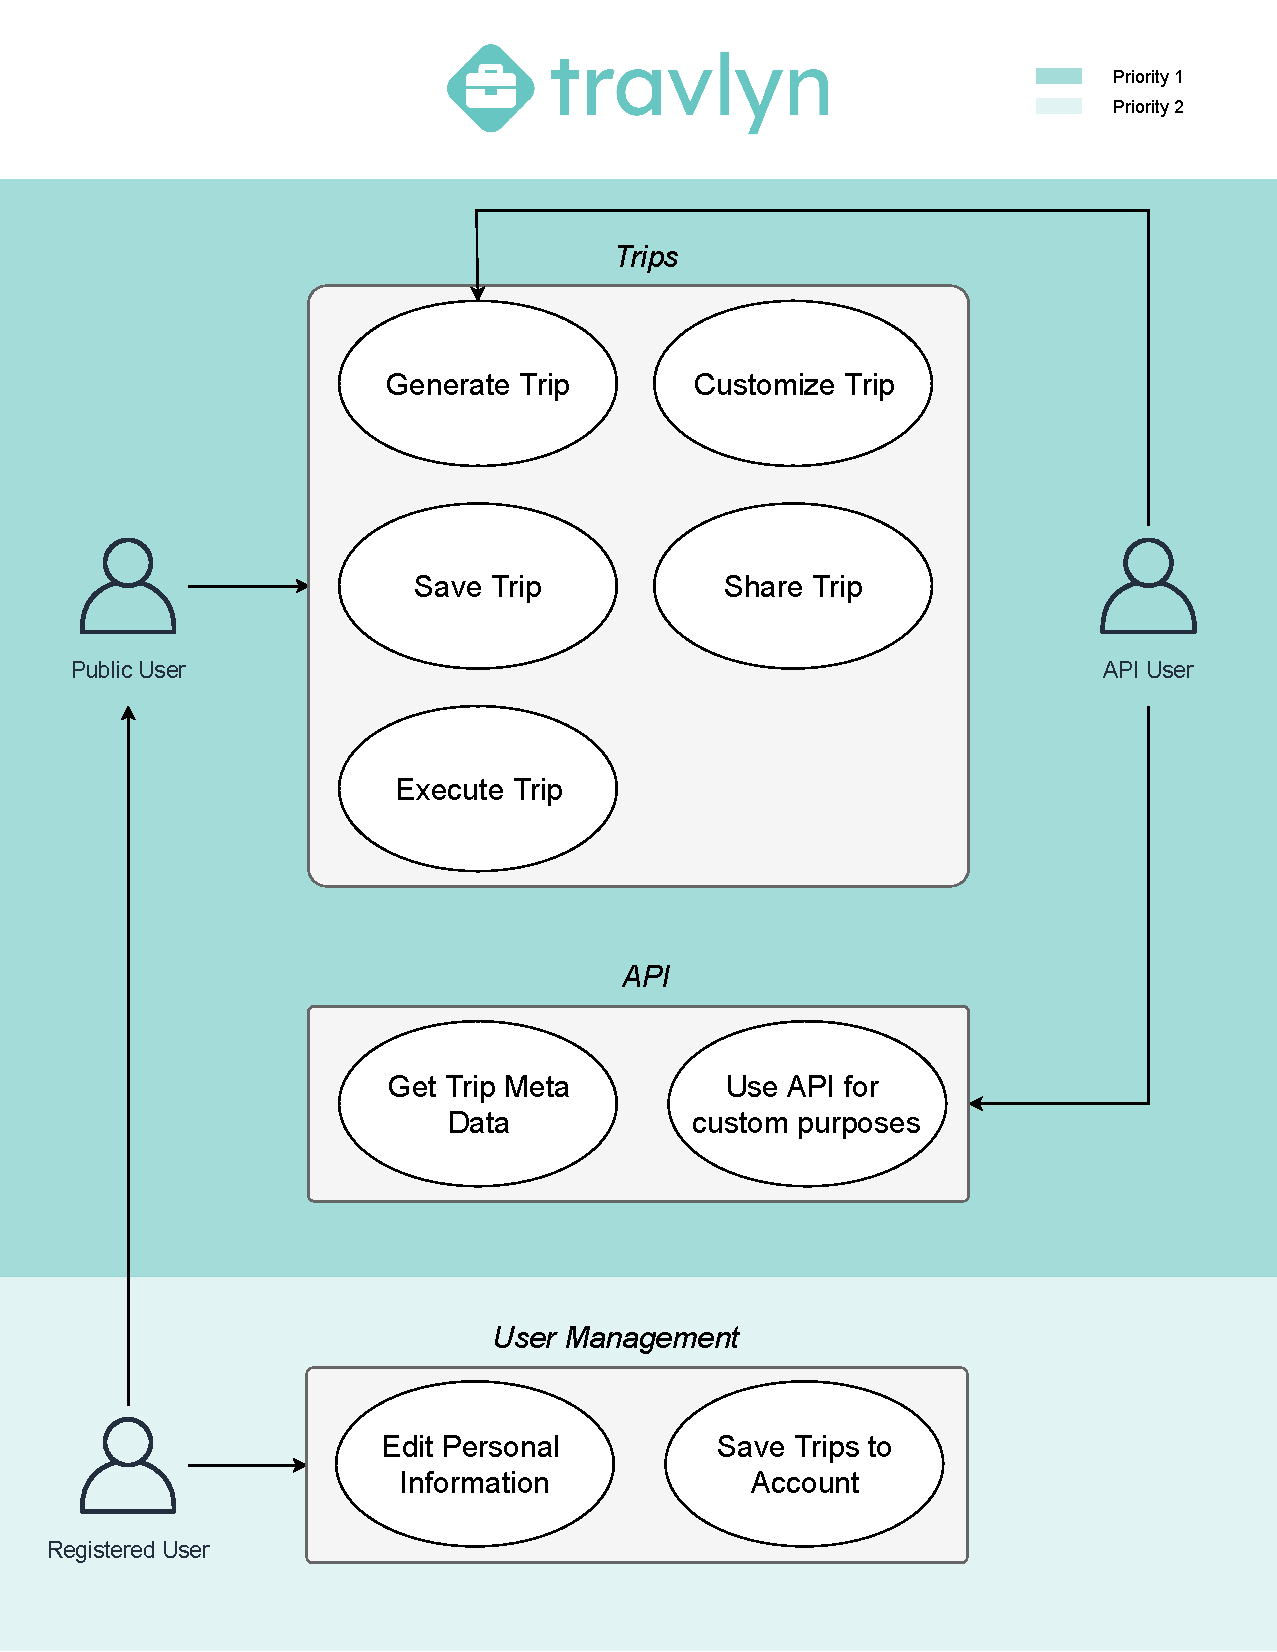
\includegraphics[width=1\textwidth]{../ucd/UCD.pdf}
	\caption{Darstellung aller geplanten Use Cases mit den assoziierten Nutzerprofilen.}
	\label{fig:UCD}
\end{figure}

\newpage

In \autoref{fig:UCD} wird der Begriff \textit{Trip} geprägt, welcher sich durch die gesamte Softwareentwicklung und Arbeit ziehen wird.

\begin{defStrich}[Trip]
	Ein Trip ist eine durch den Server erstellte Abfolge von sehenswerten Punkten in einer Stadt. Damit ist jeder Trip eindeutig einer Stadt zugeordnet. Neben den Punkten und der Route, um sich entlang der Punkte zu bewegen, werden weitere Metainformationen zu den Punkten geliefert, die einen Besuch noch interessanter machen.
\end{defStrich} 

\vspace{0.25cm}

\autoref{fig:UCD} zeigt neben den Use Cases auch die Nutzerprofile, denen die Use Cases zugeordnet sind. Für \textit{Travyln} sind vier Nutzerprofile geplant. Der \textit{interessierte Nutzer} benutzt die App eher zufällig und ohne die Intention sie aktiv für eine Reise einzusetzen. Sein Ziel ist es sich über die Funktionalität und bereits bestehende Trips zu informieren. Sollte der Nutzer in dieser Phase ansprechende Informationen finden und sich entscheiden \textit{Travyln} für die nächste Reise einzusetzen entwickelt er sich zum \textit{Öffentlichen Nutzer}, welcher ohne sich anzumelden oder zu registrieren alle Aktionen auf Trips ausführen kann und die volle Funktionalität zur Durchführung von Trips nutzt. Darauf aufbauend ist eine freiwillige Registrierung möglich, um persönliche Daten zu hinterlegen und alle eigenen Trips in an einem persönlichen Platz zu speichern. Alle Nutzer die sich dafür entscheiden liegen im Profil \textit{registrierter Nutzer}.

\vspace{0.25cm}

Da die RESTful API, die im Zuge dieser Softwareentwicklung erstellt wird, öffentlich angeboten wird, ist es möglich diese API in fremden Applikationen zu eigenen Zwecken zu nutzen. Aus diesem Anwendungsfall bildet sich das Profil \textit{API Nutzer}. Es ergeben sich aus \autoref{fig:UCD} z.B. Funktionen, wie die Abfrage von öffentlichen Trips, um diese in einer eigenen Applikation an zu bieten und als Inspiration zu Nutzen. Ein vorstellbares Szenario wäre die Nutzung auf der Website einer Stadt zu Werbezwecken. Eine weitere benutzbare Funktion wäre die Ausnutzung der in \textit{Travlyn} vorliegenden Informationssammlung für eigene Zwecke wie Machine Learning o. Ä.. 

\vspace{0.25cm}

 
Alle in \autoref{fig:UCD} dargestellten Use Cases wurden auf ihre Kompatibilität zu Zielen und Rahmenbedingungen geprüft und für passend befunden. Zusätzlich wurden sie bereits grob priorisiert. Es ist wichtig zu erwähnen, dass viele der dargestellten Use Cases im Laufe der Entwicklung zu kleinen Einheiten aufteilt werden, die hier im Sinne der Übersichtlichkeit nicht dargestellt sind.



Abschließend ist zu erwähnen, dass die funktionalen Anforderungen der in der Einführung geschilderten Funktionalität folgen soll.

\subsection{Nicht-Funktionale Eigenschaften}
Neben den geschilderten funktionalen Eigenschaften gibt es weitere Anforderungen, welche sich nicht direkt auf die Funktionalität und den Funktionalitätsumfang auswirken. Diese Eigenschaften werden auch \ac{QoS} genannt und beinhalten häufig Eigenschaften wie  Genauigkeit, Verfügbarkeit und  Konsumierbarkeit. Es ist zu erwähnen, dass einige dieser Anforderungen miteinander in Konflikt stehen und ein geeigneter Mittelweg gefunden werden muss bzw. bestimmte Kompromisse eingegangen werden müssen, z.B. schränkt die Eigenschaft der möglichst hohen Sicherheit meist die Eigenschaft der Benutzbarkeit oder der Speichereffizienz ein \cite{Balzert.2009}.  

\vspace{0.25cm}

Für diese Softwareentwicklung soll für die nicht-funktionalen Eigenschaften als Orientierung die internationale ISO/IEC 25010 Norm gelten. Diese Norm setzt einen Standard für die Qualitätskriterien und -bewertung von Software und ist in drei Bereiche aufgeteilt \cite{ISO.2011} \cite{Braun.2016}:

\begin{itemize}
	\item \textbf{Quality In Use Model}: Dieser Teil beschreibt alle Merkmale, welche die Interaktion zwischen Mensch und System beschreiben, wie z.B. Effektivität und Freiheit von Risiken.
	\item \textbf{Product Qualitiy Model}: Der zweite Teil der Norm beschreibt acht Charakteristika, welche ein Softwareprodukt erfüllen sollte, u.a. Wartbarkeit, Sicherheit und Benutzbarkeit.
	\item \textbf{Data Quality Model}: Der dritte und letzte Teil beschreibt Ansprüche, welche an das Datenmodel gestellt werden sollten um eine möglichst konsistente Benutzung der Daten zu ermöglichen.
\end{itemize}

Diese Norm ist sehr umfangreich und für ein Studienprojekt nicht vollständig umsetzbar, ohne den Zeit- und Aufwandsrahmen zu sprengen. Deshalb wurde einige wichtige Punkte ausgewählt auf die ein besonderes Augenmerk gelegt werden soll. Zusätzlich wurden einige themenspezifische Anforderungen hinzugefügt. Daraus ergibt sich folgende Liste:

\begin{itemize}
	\item \textbf{Benutzbarkeit}: Durch die intensive mobile Benutzung der \textit{Travyln} App sollte diese für alle gängigen Gerätetypen eine gute Nutzungserfahrung bieten, die Nutzer überzeugen kann und die Reise angenehm verlaufen lässt. Explizit soll an dieser Stelle die Performance der Software genannt werden, welche bei anderen Applikationen häufig für eine schlechte Benutzbarkeit sorgt. Außerdem sollen ansprechende User Interfaces gestaltet werden, die den Nutzer zur Verwendung von \textit{Travlyn} einladen und z.B. über Spracheinstellungen für möglichst viele Personen anpassbar sind.
	\item \textbf{Sicherheit}: Der Schutz persönlicher Daten wir immer wichtiger und soll auch bei \textit{Travyln} nicht vernachlässigt werden. Sowohl die API als auch die Client Applikation sollen nicht anfällig für gängige Angriffe, wie Injection oder Denial of Service Angriffe (bzw. Distributed denial of service) \cite{Mirkovic.2005} sein und sicherstellen, dass persönliche Daten nur an authentifizierte Nutzer ausgeliefert/angezeigt werden.
	\item \textbf{Wartbarkeit}: Die Software sollte über die bereits beschriebenen qualitätssichernden Maßnahmen und durch eine entsprechende Architektur gut wartbar und erweiterbar sein. Um dieses Ziel zu erreichen soll auf eine möglichst modularisierte Architektur geachtet werden. An dieser Stelle ist der Verzicht auf \textit{code ownership} besonders hervorzuheben, d.h. alle Teilnehmer des Entwicklungsteams haben Einblicke in alle Teile des Codes und können im Notfall Korrekturen und Erweiterungen vornehmen. Es ist nicht erwünscht, dass einzelne Code Teile nur von einer Person geschrieben, gepflegt und gewartet werden. Außerdem soll durch den Server eine ausführliche Dokumentation der Benutzung angefertigt werden, um auftretende Fehler identifizieren und beheben zu können. Hierzu sollen alle Aktionen und ihr Ergebnis in geeigneter Weise persistiert werden.
	\item \textbf{Datenquellen}: Da diese Software im Rahmen eines Studienprojekts mit sehr begrenzten Ressourcen erstellt wird, können keine kostenpflichtige Services eingebunden werden. Außerdem sollen schwierige Lizenzfragen vermieden werden, indem komplett auf Opensource Dienste gesetzt wird, bei denen die Nutzung der Daten vollständig erlaubt und frei ist. In den folgenden Kapiteln wird genauer auf dieses Thema eingegangen und die verschiedenen Alternativen um Daten zu beschaffen genauer vorgestellt.
	\item \textbf{Zuverlässigkeit}: Der Nutzer soll sich auf \textit{Travyln} verlassen können. Es ist wichtig, dass vor allem während einer Reise alle Funktionen zur Verfügung stehen und verhindern, dass der Nutzer alleine gelassen bzw. gezwungen wird auf andere Diensten zurückgreifen zu müssen.
	Außerdem sollten die Ausfallzeit für die API und den Client so gering wie möglich sein.
\end{itemize} 